% Set up the standalone document class
\documentclass{standalone}

% Input the preamble (<3)
% Preamble document

% Import tikz package
\usepackage{tikz}

% Import tikz libraries
\usetikzlibrary{shapes, arrows}
\usetikzlibrary{positioning, calc}

%----------- Create a fancy summing block
\tikzset{add/.style n args={4}{
		minimum width=6mm,
		path picture={
			\draw[black] 
			(path picture bounding box.south east) -- (path picture bounding box.north west)
			(path picture bounding box.south west) -- (path picture bounding box.north east);
			\node at ($(path picture bounding box.south)+(0,0.13)$)     {\tiny #1};
			\node at ($(path picture bounding box.west)+(0.13,0)$)      {\tiny #2};
			\node at ($(path picture bounding box.north)+(0,-0.13)$)    {\tiny #3};
			\node at ($(path picture bounding box.east)+(-0.13,0)$)     {\tiny #4};
		}
	}
}

%----------- Block style 1
\tikzstyle{block1} = [draw, fill=blue!20, rectangle, 
minimum height=3em, minimum width=6em, node distance=2.5cm]

%----------- Block style 2
\tikzstyle{block2} = [draw, fill=blue!20, rectangle, 
minimum height=3em, minimum width=3em, node distance=2.5cm]

%----------- Sum style
\tikzstyle{sum} = [draw, fill=blue!20, circle, node distance=2cm]

%----------- Input style
\tikzstyle{input} = [coordinate, node distance=4cm]

%----------- Output style
\tikzstyle{output} = [coordinate, node distance=4cm]

%----------- Pin style
\tikzstyle{pinstyle} = [pin edge={to-,thin,black}]

\begin{document}

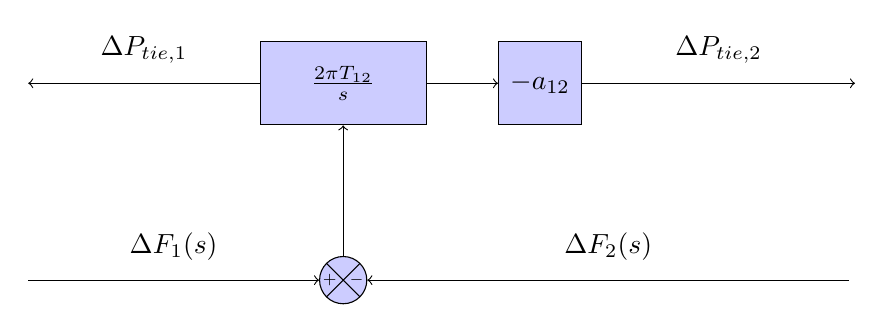
\begin{tikzpicture}
	
	% Draw the nodes first
	\node [input] (input1) {};
	\node [sum,add={ }{+}{ }{$-$}, right of=input1, node distance=4cm] (sum) {};
	\node [right of=sum, node distance=6.55cm] (input2) {};
	\node [block1, above of=sum] (tieline) {$\frac{2 \pi T_{12}}{s}$};
	\node [block2, right of=tieline] (a12) {$-a_{12}$};
	\node [output, right of=a12] (P2) {};
	\node [output, left of=tieline] (P1) {};
	
	% Connect the nodes
	\draw [->] (input1) -- node [label=above:{$\Delta F_1(s)$}] {} (sum);
	\draw [->] (input2) -- node [label=above:{$\Delta F_2(s)$}] {} (sum);
	\draw [->] (sum) -- (tieline);
	\draw [->] (tieline) -- node[label=above:{$\Delta P_{tie,1}$}] {} (P1);
	\draw [->] (tieline) -- (a12);
	\draw [->] (a12) -- node[label=above:{$\Delta P_{tie,2}$}] {} (P2);
\end{tikzpicture}

\end{document}
